\documentclass[11pt]{article}

\usepackage[margin=1in, headheight=14.5pt]{geometry}
\usepackage{amsfonts, amsmath, amssymb}
\usepackage[none]{hyphenat}
\usepackage{fancyhdr}
\usepackage[spanish]{babel}
\usepackage[spanish, calc]{datetime2}
\usepackage{fmtcount}
\usepackage{graphicx}
\usepackage{float}
\usepackage[nottoc, notlot, notlof]{tocbibind}
\usepackage{tocloft}
\usepackage[utf8]{inputenc}
\usepackage{parskip}
\usepackage{xcolor}
\usepackage{cancel}
\usepackage{textcomp}
\usepackage{pgfplots}
\usepackage{tikz}
\usetikzlibrary{datavisualization}
\usetikzlibrary{datavisualization.formats.functions}
\pgfplotsset{compat=1.15}
\usepackage{mathrsfs}
\usetikzlibrary{arrows}
\usepackage{mathtools}

\parindent 0ex

\pgfplotsset{width=10cm,compat=1.9}

\def\imj{\mathrm{j}}
\def\sen{\mathrm{sen}}

\renewcommand\cftsecleader{\cftdotfill{\cftdotsep}}
\renewcommand{\baselinestretch}{1.1}
\newcommand*\circled[1]{\tikz[baseline=(char.base)]{
		\node[shape=circle,draw,inner sep=2pt] (char) {#1};}}

\graphicspath{{C:/Users/tomas/OneDrive/Escritorio/LATEX/matematica-superior/commons/img/}}

\pagestyle{fancy}
\fancyhead{}
\fancyfoot{}
\fancyhead[L]{\MakeUppercase{Matemática Superior}}
\fancyhead[R]{\slshape Series de Fourier: Ejercicios de final}
\fancyfoot[C]{\thepage}


\begin{document}
		
	\begin{titlepage}
		\begin{center}
			\vspace*{0.5cm}
			\Large{\textbf{Universidad Tecnológica Nacional}}\\
			\Large{\textbf{Facultad Regional Buenos Aires}}\\
			\begin{center}
				
\includegraphics[scale=0.4]{logoutn.png}
			\end{center}
			\vfill
			\line(1,0){400}\\
			\vspace*{0.3cm}
			\huge{\textbf{Matemática Superior}}\\
			\Large{\textbf{Unidad 2: Series de Fourier}}\\
			\large{Ejercicios resueltos de final}
			\line(1,0){400}\\
			\vfill
			Tomás Moreira \\
			
			\DTMnewdatestyle{mydate}{%
				\renewcommand{\DTMdisplaydate}[4]{%
					\DTMMonthname{##2} \number##1
				}
				\renewcommand{\DTMDisplaydate}{\DTMdisplaydate}
			}
			
			\DTMsetdatestyle{mydate}
			\today
				
				
		\end{center}
	\end{titlepage}

	\tableofcontents
	\thispagestyle{empty}
	\clearpage

	\setcounter{page}{1}
	\section{Introducción}
	Esta recopilación está tomada de algunos finales que están disponibles en el aula virtual general de la materia, y algunos son de finales más nuevos (2018-2020). Se pretende dar una solución con detalle, y remarcar algunos errores comunes, y recomendaciones para encarar los distintos ejercicios. Espero que te sea útil, y cualquier pregunta, no dudes en consultar en el aula virtual!
	\section{Ejercicio 1}
	Final 19/12/2017. \textit{Elegir la respuesta correcta}:\\
	Dada la función $f(x)=e^{x}-1$ en $\left[0,1\right)$, para que tenga simetría de media onda con período $T=2$ hay que definirla en $\left[1,2\right)$:
	\renewcommand{\labelenumi}{\alph{enumi})}
	\begin{enumerate}
		\item $f(x)=-e^{x}+1$
		\item $f(x)=-e^{x-1}+1$
		\item $f(x)=-e^{x-1}-1$
		\item Ninguna de las anteriores.
	\end{enumerate}

	\textbf{Resolución:}
	
	Empecemos graficando nuestra función:\\
	\begin{center}
		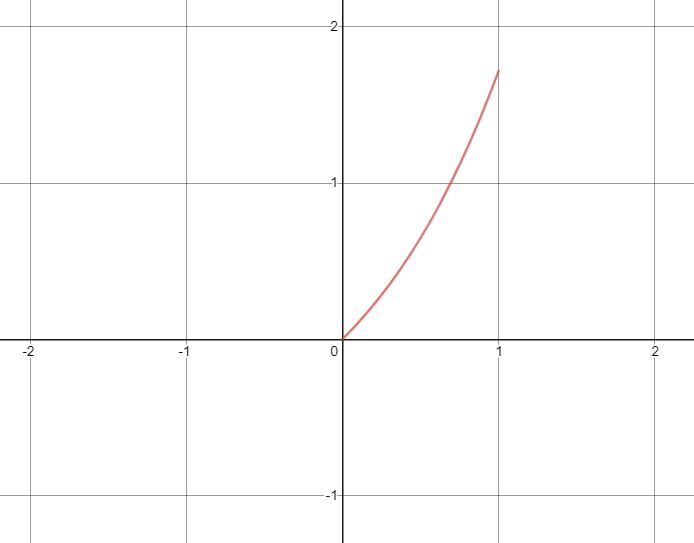
\includegraphics[scale=0.6]{02-SerieYTransformadaDeFourier/final1_1.JPG}
	\end{center}

	Podemos realizar el ejercicio en forma gráfica. Para ello, como sabemos que nuestro período de la nueva función será $T=2$, tenemos que desplazar nuestra función medio período (es decir, graficarla en el $(1,2)$) y luego espejarla con respecto al eje de abscisas, de la siguiente manera:\\
	
	\begin{center}
		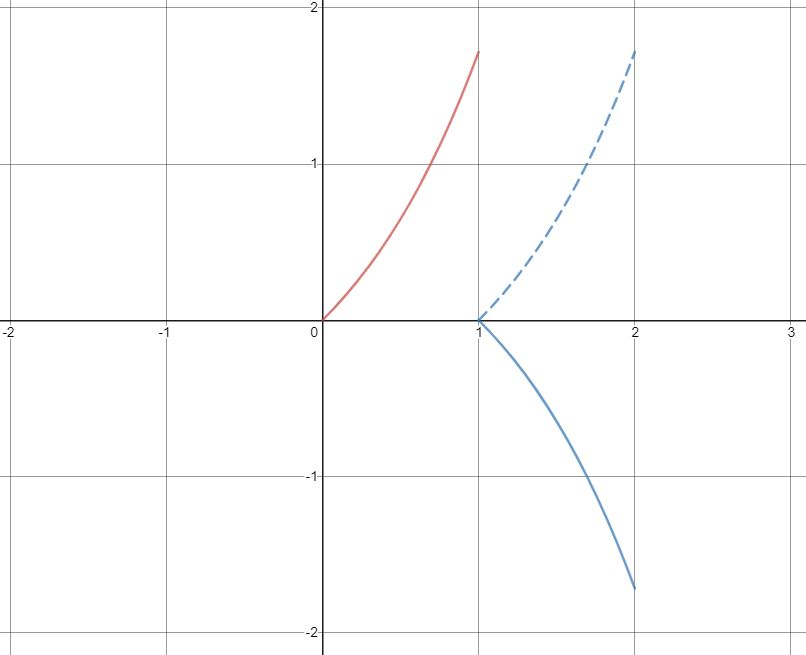
\includegraphics[scale=0.6]{02-SerieYTransformadaDeFourier/final1_2.JPG}
	\end{center}

	Luego, sería cuestión de deducir la forma de la función.
	
	En forma analítica, podemos usar la definición de función con simetría de media onda:	
	$$f(x)=-f(x+L)$$ Donde $L$ es el semiperiodo, es decir $T/2$.
	
	En nuestro caso sabemos que $T=2$, por ende $L=1$, aunque como el otro trozo de función lo piden en un desplazamiento hacia la derecha, vamos a tomarnos el atrevimiento de usar $f(x)=-f(x-L)$. En nuestro caso, $f(x)=-f(x-1)$
	
	Reemplazamos: $f(x)=-\left(e^{(x-1)}-1\right)$
	
	Distribuimos y sacamos los paréntesis redundantes, llegando a la función en forma analítica:\\
	$\boxed{f(x)=-e^{x-1}+1}$
	
	Por lo tanto, \fcolorbox{black}{yellow}{la respuesta correcta es la \textbf{\underline{b}}}.
	\section{Ejercicio 2}
	Final 22/02/2018. \textit{Indicar verdadero o falso}:\\
	La función $   
	f(x) = 
	\begin{cases}
	5 &\quad\text{si}\;-2\leq x \leq 2\\
	2 &\quad\text{si}\;\;2< |x| < 3 \\
	\end{cases}
	\enspace\wedge\enspace
	f(x)=f(x+6)
	$
	tiene valor medio $4$.
	
	\textbf{Resolución:}
	
	Primero, realicemos un gráfico de la función:
	\begin{center}
		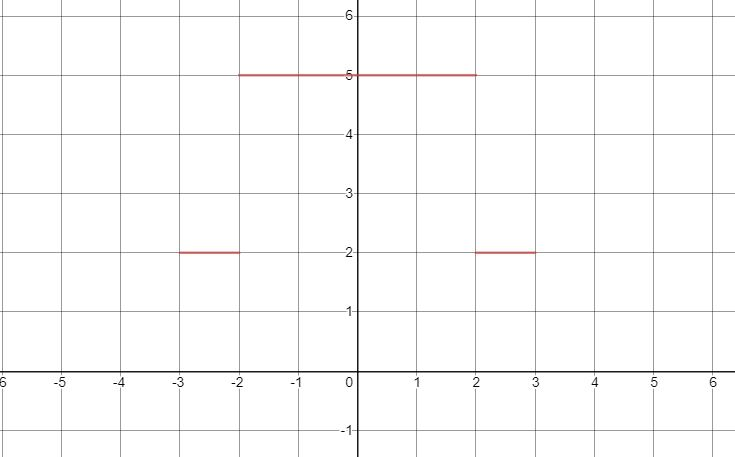
\includegraphics[scale=0.6]{02-SerieYTransformadaDeFourier/final2_1.JPG}
	\end{center}

	Rápidamente, podríamos reducirnos al truco de ``contar cuadraditos" de una hoja cuadriculada, siempre que hagamos la gráfica a la escala:
	\begin{center}
		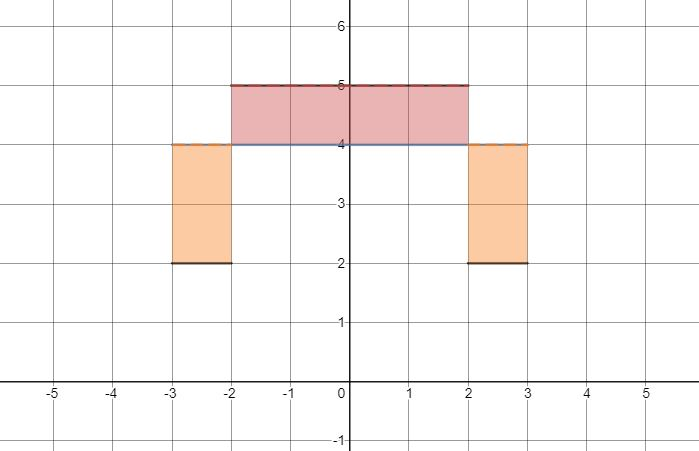
\includegraphics[scale=0.6]{02-SerieYTransformadaDeFourier/final2_2.JPG}
	\end{center}

	Y concluiríamos diciendo que el área encerrada entre ambos trozos de la función y el valor medio es la misma (y vale 4).
	
	De todos modos, recuerden que siempre se puede hacer la integral para verificar el resultado. En este caso es fácil de visualizar de forma gráfica.
	
	\fcolorbox{black}{yellow}{Respuesta: \textbf{\underline{VERDADERO}}}
	\pagebreak
	
	\section{Ejercicio 3}
	Final 15/02/2018. \textit{Indicar verdadero o falso}:\\
	Al desarrollar la función $f(t)=\sen\left(\pi t\right)$ si $t\in(0,1) \wedge f(t)=f(t+1)$ en Serie Exponencial de Fourier sólo hay términos con coeficientes reales.
	
	\textbf{Resolución:}
	
	Como no nos piden que desarrollemos la Serie, vamos a justificar la respuesta con fundamentos teóricos.
	
	Primero, hay que tener muchísimo cuidado y analizar muy bien la función que nos dan, y siempre hacer un gráfico.\\
	Cualquiera podría pensar que si nos están dando un seno, que es una función impar, ya podríamos dar la respuesta sin analizar nada. Pero en este caso no es así, hay que ver que forma tiene nuestra función y también revisar con cuidado el período donde está definida.
	
	Procedamos a graficar el trozo de función que nos están planteando: \\
	\begin{center}
		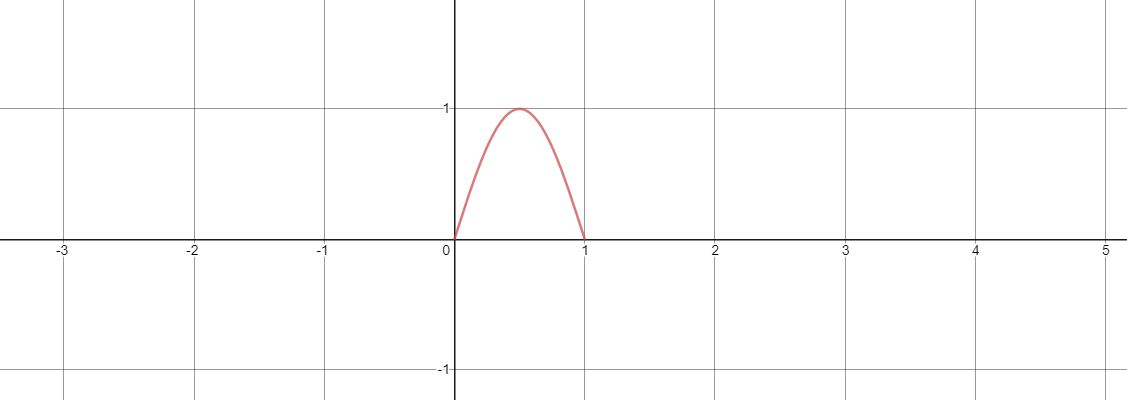
\includegraphics[scale=0.5]{02-SerieYTransformadaDeFourier/final3_1.jpg}
	\end{center}

	Como esta función es definida periódica, vamos a graficar algunos trozos más:
	\begin{center}
		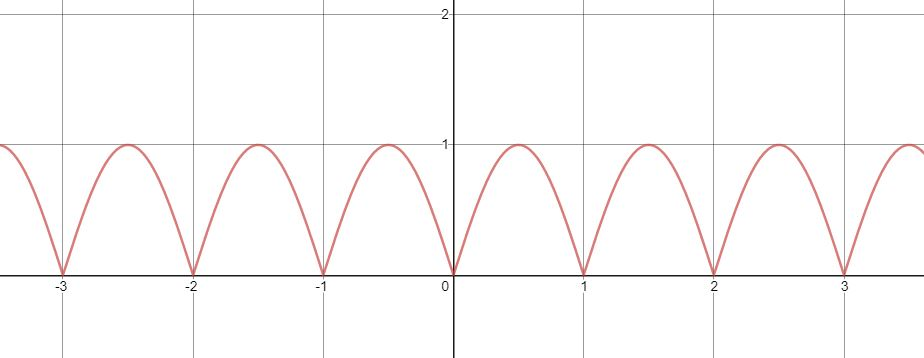
\includegraphics[scale=0.5]{02-SerieYTransformadaDeFourier/final3_2.jpg}
	\end{center}

	Miren que interesante, visualizando el gráfico, a pesar de ser la función un seno, y por como está definida, resulta ser par!
	
	Por lo tanto, los $b_{n}$ van a ser $0$.
	
	Recordemos una manera de calcular los coeficientes de la SEF: $c_{n}=\frac{a_{n}-b_{n}\imj}{2}$
	
	Por ende, sabiendo que $b_{n}=0$, los coeficientes terminarán siendo todos reales.
	
	\fcolorbox{black}{yellow}{Respuesta: \textbf{\underline{VERDADERO}}}
	\section{Ejercicio 4}
	Final 12/12/2017. \textit{Indicar la respuesta correcta}:\\
	La Serie Exponencial de Fourier de $f(x)=4-x$ si $x\in(0,2) \wedge f(x)=f(x+2)$ tiene los coeficientes:
	\renewcommand{\labelenumi}{\alph{enumi})}
	\begin{enumerate}
		\item Todos reales.
		\item Todos imaginarios.
		\item Uno real y resto imaginarios.
		\item Ninguna de los anteriores.
	\end{enumerate}

	\textbf{Resolución:}
	
	Como siempre, vamos a comenzar realizando una gráfica:
	\begin{center}
		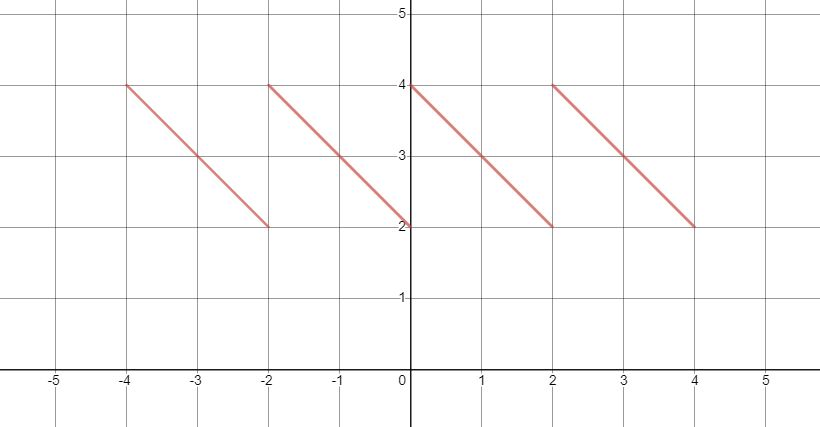
\includegraphics[scale=0.4]{02-SerieYTransformadaDeFourier/final4_1.jpg}
	\end{center}

	Bien, en principio esta función no es ni par ni impar si miramos el gráfico. \\
	Sin embargo, si observamos con detenimiento, no está muy lejos de ser una función impar. Pensemos en la siguiente gráfica (la de líneas punteadas):
	
	\begin{center}
		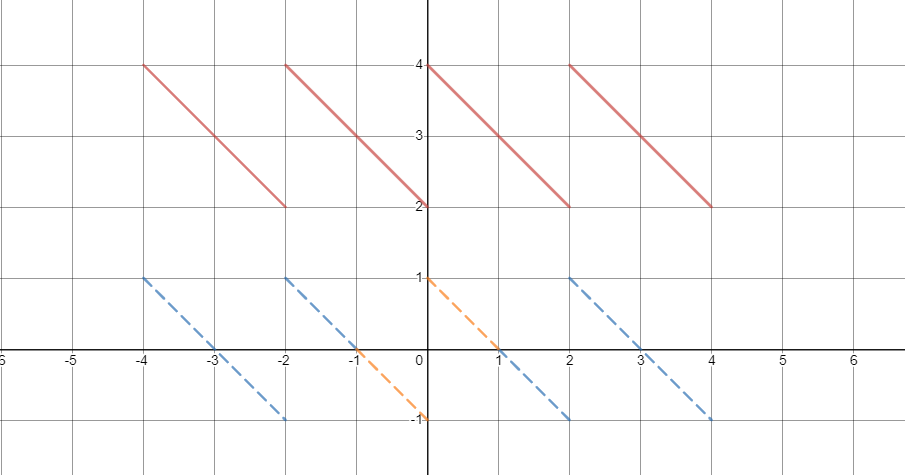
\includegraphics[scale=0.53]{02-SerieYTransformadaDeFourier/final4_2.jpg}
	\end{center}

	La función graficada en líneas punteadas es impar, eso se ve claramente en el período que va desde $-1$ a $0$ y de $0$ a $1$ (que es el marcado en naranja). 
	
	De hecho, es la función $g(x)=1-x$ en $(0,2) \wedge g(x)=g(x+2)$. Comparando tanto las gráficas, como la definición de las funciones, podemos ver claramente que $f(x)=g(x) + 3$
	
	Luego, si llamamos $Sf(x)$ al desarrollo en serie de la función f, este se podría calcular como:\\ $Sf(x)=Sg(x)+3$
	
	Por lo tanto, podríamos pensar a la función del ejercicio como la suma de una función impar y una constante, por ende, la serie solo va a diferir en el término independiente.
	
	Considerando todo esto, podemos concluir que la \fcolorbox{black}{yellow}{respuesta correcta es la \textbf{\underline{c}}}.
	\section{Ejercicio 5}
	Final 07/10/2016. \textit{Desarrollar}:\\
	El desarrollo de $f(x)=x+3$ si $x\in(-1,1)\wedge f(x)=f(x+2)$ en Serie Trigonométrica de Fourier es:\\
	$S(x)=_{\;\cdots\cdots\cdots\cdots\cdots\cdots\cdots\cdots\cdots\cdots\cdots\cdots\cdots\cdots\cdots\cdots\cdots\cdots\cdots\cdots\cdots\cdots\cdots\cdots\cdots}$
	
	\textbf{Resolución:}
	
	En este ejercicio nos toca calcular la serie, por ende, hay que recurrir a las integrales!
	
	Empecemos primero por el gráfico:
	\begin{center}
		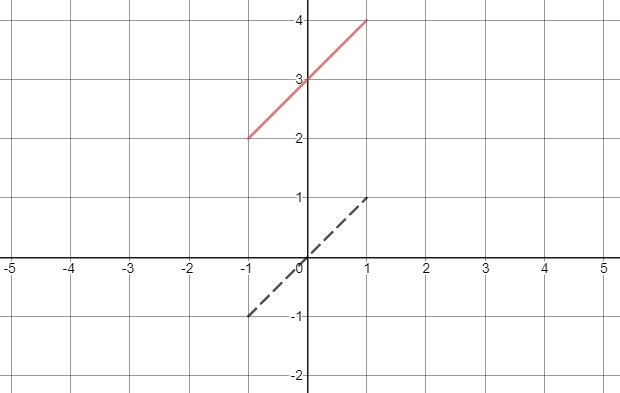
\includegraphics[scale=0.7]{02-SerieYTransformadaDeFourier/final5_1.jpg}
	\end{center}

	La roja es la función del ejercicio, y la línea punteada es el reflejo de lo discutido en el ejercicio anterior. La función del ejercicio resulta ser impar desplazada en 3 unidades hacia arriba. Por ende si llamamos $g(x)=x$ podemos decir $f(t)=g(t)+3\;$ \textrightarrow $\;Sf(t)=Sg(t)+3$, entonces conviene calcular la serie para $g(x)=x$ y luego le sumamos la constante.
	
	Luego, para $g$, al ser impar, tenemos que $a_{0}=a_{n}=0$
	
	Entonces procedemos a calcular los $b_{n}$:
	
	Obtenemos los elementos notables: $T=2$, $L=1$, $\omega=\frac{\pi}{L}=\pi$
	
	$\displaystyle b_{n}= \frac{1}{L} \int_{-L}^{L} g(x)\sen(n\omega x) dx$
	
	Pero como se aprendió en la teoría, podemos reescribirla como:
	
	$\displaystyle b_{n}= \frac{2}{L} \int_{0}^{L} g(x)\sen(n\omega x) dx$
	
	Reemplazamos nuestros valores:
	
	$\displaystyle b_{n}= \frac{2}{1} \int_{0}^{1} x\sen(n\pi x) dx=2\left[\frac{\sen(n\pi x)}{n^2\pi^2}-\frac{x\cos(n\pi x)}{n\pi}\right]_{0}^{1}$
	
	Evaluamos:
	
	$\displaystyle b_{n}=2\left[\frac{\sen(n\pi)}{n^2\pi^2} - \frac{\cos(n\pi)}{n\pi} - \frac{\sen(0)}{n^2\pi^2} + \frac{0\cos(0)}{n\pi}\right]=\displaystyle b_{n}=2\left[\frac{\sen(n\pi)}{n^2\pi^2} - \frac{\cos(n\pi)}{n\pi}\right]$
	
	Ahora, analizando un poco los términos con coseno y seno, recordemos lo siguiente:
	
	Teniendo en cuenta que $n$ es un número natural: \\
	$\cos(\pi)=-1 \quad \cos(2\pi)=1 \quad \cos(3\pi)=-1 \quad \cos(4\pi)=1$\\
	$\sen(\pi)=0 \quad \sen(2\pi)=0 \quad \sen(3\pi)=0 \quad \sen(4\pi)=0$
	
	Por ende para los cosenos, podemos reemplazar $\cos(n\pi)$ por $(-1)^{n}$, y para los senos, directamente por $0$.
	
	La expresión queda entonces: $\displaystyle b_{n}=-\frac{2(-1)^n}{n\pi}$
	
	La serie de $g$ es entonces: $\displaystyle Sg(x)=\sum_{n=1}^{\infty}-\frac{2(-1)^n}{n\pi} \sen(n\pi x)$
	
	Sin embargo, recordemos que nosotros en realidad buscamos la serie para $f$ !!!! Así que recordar lo que habíamos planteado al principio: $Sf(x)=Sg(x)+3$
	
	Por último: \fcolorbox{black}{yellow}{$\displaystyle Sf(x)=S(x)=3+ \sum_{n=1}^{\infty}-\frac{2(-1)^n}{n\pi} \sen(n\pi x)$}
	\section{Ejercicio 6}
	Final 12/05/2015. \textit{Desarrollar}:\\
	Dada la función $   
	f(x) = 
	\begin{cases}
	4 &\quad\text{si}\;-1< x < 1\\
	k &\quad\text{si}\;\;1< x < 5 \\
	\end{cases}
	\enspace\wedge\enspace
	f(x)=f(x+6)
	$:
	\renewcommand{\labelenumi}{\alph{enumi})}
	\begin{enumerate}
		\item Calcule el valor de $k\in\mathbb{R}$ para que el valor medio de $f(x)$ sea $3$.
		\item Con $k=0$, obtenga la Serie Trigonométrica de Fourier.
		\item En base al punto anterior, obtenga la Serie Exponencial de Fourier.
	\end{enumerate}

	\textbf{Resolución:}
	
	a) Para realizar esta parte, vamos a recurrir primero al cálculo por la integral.
	
	Sabemos que $\displaystyle \frac{a_{0}}{2}=3$
	
	Entonces, recuerden que $a_{0}=\displaystyle \frac{1}{L} \int_{-L}^{L}f(x)dx$
	
	Calculemos entonces el $a_{0}$ para lo que tenemos: $\displaystyle a_{0}= \frac{1}{3} \int_{-1}^{1} 4dx + \frac{1}{3} \int_{1}^{5}kdx$\\
	$\displaystyle a_{0}=\frac{4}{3} \left(1+1\right) + \frac{k}{3} \left(5-1\right)=\frac{8+4k}{3}$
	
	Luego, $\displaystyle \frac{a_{0}}{2}=3\;$ \textrightarrow $\;\displaystyle 3=\frac{8+4k}{6}\;$ \textrightarrow $\;18=8+4k \;$ \textrightarrow \fcolorbox{black}{yellow}{$k=2.5$}
	
	Luego, habríamos terminado este inciso.
	
	Sin embargo, me gustaría discutir otro tema antes de pasar al siguiente inciso. Sabemos ya que al valor medio lo podemos obtener observando el gráfico.
	
	Analicemos este caso y grafiquemos lo que conocemos:
	\begin{center}
		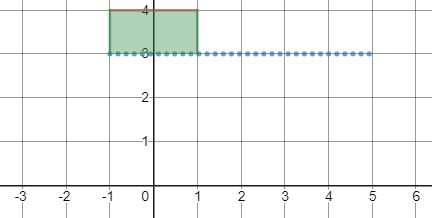
\includegraphics[scale=1]{02-SerieYTransformadaDeFourier/final6_1.jpg}
	\end{center}

	Puede pasar que, por hacerlo mecánicamente, uno ve el enunciado y dice: ``el otro pedazo debe valer 2 seguro" (porque además nos dicen que es una constante).
	
	Sin embargo hay que tener mucho cuidado con sacar estas conclusiones de forma rápida, como vimos en el resultado haciendo la integral, el valor de $k$ terminó siendo $2.5$.
	
	Esto pasa porque el trozo que va de -1 a 1 no ocupa la mitad del período, por ende si proponemos que el valor de $k$ sea 2, nos van a quedar desproporcionadas las áreas. En este caso, podemos seguir haciendo el cálculo geométricamente, sabiendo que son rectángulos ambas áreas.
	
	Sabemos que el primer trozo tiene área igual a 2. Mientras que para el otro trozo, sabemos que su base es 4, por lo tanto si $A=b\cdot h$, entonces necesariamente la altura debe ser $0.5$.
	
	Luego, se concluye que \fcolorbox{black}{yellow}{$k=2.5$}.
	
	Gráfica:
	\begin{center}
		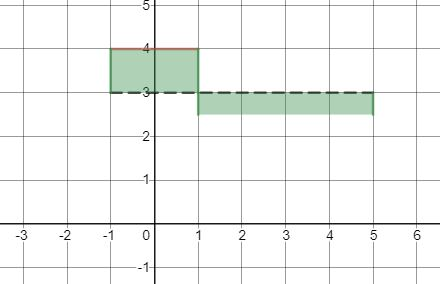
\includegraphics[scale=1]{02-SerieYTransformadaDeFourier/final6_2.jpg}
	\end{center}

	b) Como $k=0$, entonces la función queda definida:
	
	$   
	f(x) = 
	\begin{cases}
	4 &\quad\text{si}\;-1< x < 1\\
	0 &\quad\text{si}\;\;1< x < 5 \\
	\end{cases}
	\enspace\wedge\enspace
	f(x)=f(x+6)
	$
	
	Su gráfica, por ende:\\
	\begin{center}
		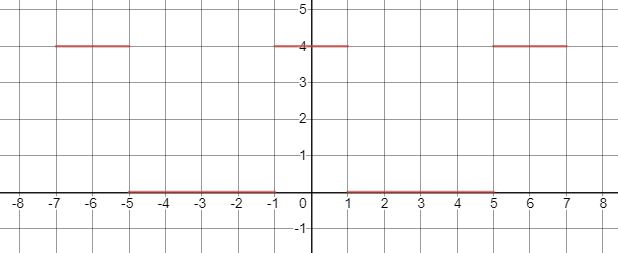
\includegraphics[scale=1]{02-SerieYTransformadaDeFourier/final6_3.jpg}
	\end{center}
	
	Se ve claramente que la función es par, por ende $b_{n}=0$
	
	Anotemos los valores notables: $T=6, \; L=3, \; \omega=\frac{\pi}{3}$
	
	Ahora calculemos los coeficientes:
	
	$\displaystyle a_{0}=\frac{2}{3}\int_{0}^{1}4dx=\frac{8}{3}\implies\frac{a_{0}}{2}=\frac{4}{3}$
	
	$\displaystyle a_{n}=\frac{2}{3}\int_{0}^{1}4\cos\left(n\frac{\pi}{3}x\right)dx=\frac{8}{3}\left[\frac{\sen\left(n\frac{\pi}{3}x\right)}{n\frac{\pi}{3}}\right]_{0}^{1}=\boxed{\frac{8}{n\pi}\sen\left(n\frac{\pi}{3}\right)}$
	
	Por último, armamos la serie:\\
	\fcolorbox{black}{yellow}{$\displaystyle S(x)=\frac{4}{3}+\sum_{n=1}^{\infty}\frac{8}{n\pi} \sen\left(n \frac{\pi}{3}\right) \cos\left(n\frac{\pi}{3}x\right)$}
	
	c) Para esto, simplemente hay que recordar que:
	
	$\displaystyle c_{n}=\frac{a_{n}-b_{n}\imj}{2}\;$ \textrightarrow $\displaystyle \;\boxed{c_{n}=\frac{4}{n\pi}\sen\left(n\frac{\pi}{3}\right)}$
	
	La serie exponencial queda conformada entonces:
	
	\fcolorbox{black}{yellow}{$\displaystyle S(x)=\frac{4}{3}+\sum_{\mathclap{\substack{n=-\infty \\ n\neq0}}}^{\infty} \frac{4}{n\pi} \sen\left(n\frac{\pi}{3}\right) e^{\imj n\frac{\pi}{3}x}$}
	
	
	\section{Ejercicio 7}
	Final 27/02/2020. \textit{Indicar la respuesta correcta}:\\
	Sea la función $f(x)$ tal que $f(x)=f(x+T) \wedge f(x)=2x\cdot g(x)$ con $g(x)\neq0 \wedge g(x)$ par. La Serie Trigonométrica de Fourier es:
	\renewcommand{\labelenumi}{\alph{enumi})}
	\begin{enumerate}
		\item Solo de senos.
		\item Solo de cosenos.
		\item Con senos y cosenos.
		\item Constante.
	\end{enumerate}

	\textbf{Resolución:}
	Este ejercicio es puramente teórico.
	
	Se razona con propiedades de la paridad de funciones. Sabemos que $g$ es par, y sabemos que $2x$ es una función impar. \\
	Luego, el producto de una función par y una función impar da como resultado una función impar.
	
	Y como sabemos, si tenemos una función impar tiene su desarrollo en serie trigonométrica con solo senos.
	
	\fcolorbox{black}{yellow}{Respuesta: \textbf{\underline{a}}}
\end{document}
